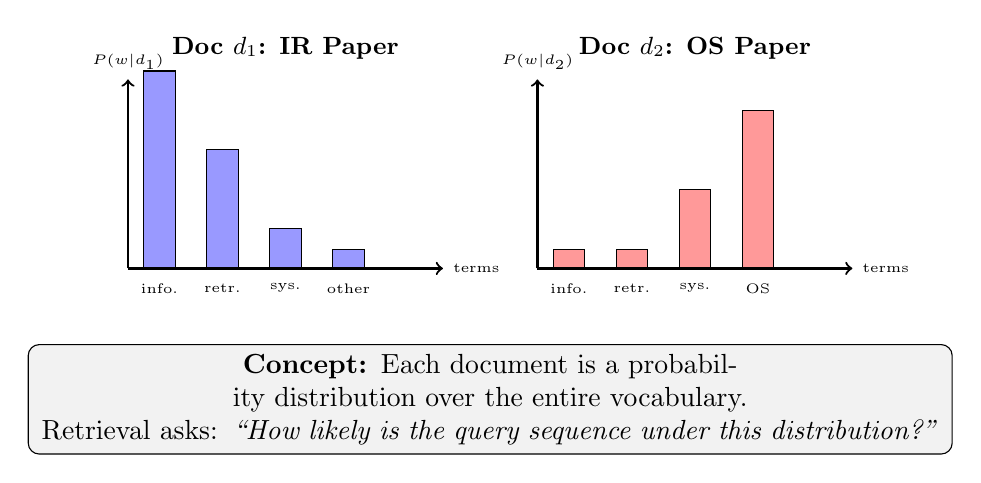
\begin{tikzpicture}[
    scale=0.8,
    bar/.style={rectangle, draw, fill=blue!40, minimum width=0.4cm, anchor=south},
    axis/.style={->, thick}
]
    % Document 1 Distribution
    \begin{scope}[xshift=0cm]
        \draw[axis] (0,0) -- (5,0) node[right] {\tiny terms};
        \draw[axis] (0,0) -- (0,3) node[above] {\tiny $P(w|d_1)$};
        \node[bar, minimum height=2.5cm] (b11) at (0.5,0) {}; % "information"
        \node[bar, minimum height=1.5cm] (b12) at (1.5,0) {}; % "retrieval"
        \node[bar, minimum height=0.5cm] (b13) at (2.5,0) {}; % "system"
        \node[bar, minimum height=0.2cm] (b14) at (3.5,0) {}; % "other"
        \node[below, font=\tiny, yshift=-2pt] at (0.5,0) {info.};
        \node[below, font=\tiny, yshift=-2pt] at (1.5,0) {retr.};
        \node[below, font=\tiny, yshift=-2pt] at (2.5,0) {sys.};
        \node[below, font=\tiny, yshift=-2pt] at (3.5,0) {other};
        \node[font=\small\bfseries] at (2.5,3.5) {Doc $d_1$: IR Paper};
    \end{scope}

    % Document 2 Distribution
    \begin{scope}[xshift=6.5cm]
        \draw[axis] (0,0) -- (5,0) node[right] {\tiny terms};
        \draw[axis] (0,0) -- (0,3) node[above] {\tiny $P(w|d_2)$};
        \node[bar, minimum height=0.2cm, fill=red!40] (b21) at (0.5,0) {}; % "information"
        \node[bar, minimum height=0.1cm, fill=red!40] (b22) at (1.5,0) {}; % "retrieval"
        \node[bar, minimum height=1.0cm, fill=red!40] (b23) at (2.5,0) {}; % "system"
        \node[bar, minimum height=2.0cm, fill=red!40] (b24) at (3.5,0) {}; % "OS"
        \node[below, font=\tiny, yshift=-2pt] at (0.5,0) {info.};
        \node[below, font=\tiny, yshift=-2pt] at (1.5,0) {retr.};
        \node[below, font=\tiny, yshift=-2pt] at (2.5,0) {sys.};
        \node[below, font=\tiny, yshift=-2pt] at (3.5,0) {OS};
        \node[font=\small\bfseries] at (2.5,3.5) {Doc $d_2$: OS Paper};
    \end{scope}

    % Descriptive Box below everything
    \node[draw, fill=gray!10, rounded corners, text width=11.5cm, align=center, anchor=north] at (5.75,-1.2) {
        \textbf{Concept:} Each document is a probability distribution over the entire vocabulary. \\
        Retrieval asks: \emph{``How likely is the query sequence under this distribution?''}
    };

\end{tikzpicture}
